\section{A Precise Method Concerning Propitious and Impropitious Times with Reference to the Rising Times and the Periods of the Stars (4K,5P)}

The same procedure must be observed with respect to propitious and impropitious times: after the yearly periods, allot the monthly periods to the operative signs and to their houserulers. Just as when we construct scientific astronomical tables, we use integer numbers and smaller fractions in order to make a sold structure; but we see that the structure is not consistent if the starting point of the numeration is not
clearly established. In the same way, one who wishes to go through a nativity accurately must begin with the hours and months, then bring the chronocratorships (in all their variety) up to the transfer of the
chronocratorship at the time in question. In so doing we will find that one star is chronocrator according to the rising times, another is chronocrator according to the stars’ periods, and that even though \textbf{/275K/} the results as a whole seem to be good or bad, in the intervening days and months the opposite may occur, and perhaps the events may seem to happen earlier or later $<$than predicted$>$. Just as a stone hurled against some skillfully-crafted bronze object hits it only momentarily, but its clang echoes for quite some time—in the same way, when the stars are chronocrators, they display their causative effects only briefly, but during the succeeding periods they are active, just like the clang. 

The \textbf{/263P/} configurations of the stars and their aspects with each other (especially the aspects with the Lot of Fortune) are effective in the chronocratorships which are in harmony. (The whole is seen and arises from the aspects of the Lot of Fortune and from its ruler.)

\newpage
For example: \Sun, \Mercury\xspace in \Gemini, \Moon\xspace in \Aquarius, \Saturn, \Venus\xspace in \Leo, \Jupiter\xspace in
\Sagittarius, \Mars, Ascendant in \Libra, klima 1\footnote{\textit{Greek Horoscopes} dates the chart to June 12, 122 CE about 2 p.m.}. 

\begin{wrapfigure}[14]{R}{7cm}
\centering
\vspace{-10pt}
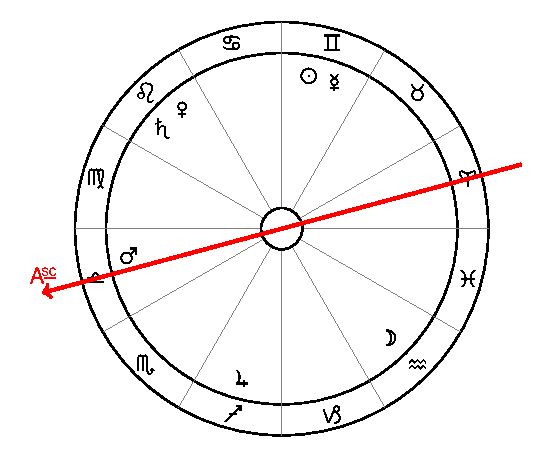
\includegraphics[width=.68\textwidth]{charts/7_5_1}
\caption{Chart 81 [VII.5.1, GH 122, VI.12]}
\label{fig:chart81}
\end{wrapfigure} 

Assume we are investigating the 42nd year. I took the rising time of \Libra, 38;20 (which is 38 years 4 months) plus the same number of months, 38 (which is 3 years 2 months). The total is 41 years 6 months. In that year while fleeing from battle, he fell from his horse as the enemy were approaching. Although many were killed and he himself was wounded, he was entangled with the rest of the slain, pretended to be dead, and escaped the danger. He then remained in the enemy’s country until his 44th year leading the campaign. To the previous number of years I added 8 months for \Venus\xspace (because of Libra) and 15 months for \Mars\xspace because it was there also $<$in \Libra$>$. In addition, the opposition of \Saturn\xspace and the \Moon\xspace was operative at that time. The rising time of \Leo, 35, plus 57 months for \Saturn, plus 8 months for \Venus, plus 25 months for the \Moon\xspace plus 19 months for \Leo\xspace $<$=\Sun$>$ together total 44 years, 1 month. 

As a result, it is necessary to give the total of rising times or of periods for the length of the nativity, then the months and days, until the forecast is made for the exact period of time. Therefore, one must observe for every nativity the stars in square and in opposition, particularly when malefics are in inappropriate configurations. In such a case, the native will be involved in all kinds of inescapable troubles. Such a man will struggle all his life, wrestling against crises hard to overcome; he will be inclined to slip and come crashing down, \textbf{/276K/} and he will easily fail. If malefics behold $<$the chronocrator$>$, such a man does not shrink from criticizing the gods; he lives wretchedly, begging for death—but in vain, unless some aspect of the benefics is effective in helping him. 

Now whenever a benefic is operative with a malefic, the bad influence will he halved and easily remedied. If one or the other is by itself, it indicates that its effects will be definite and complete, because \textbf{/264P/} a good effect is hindered and overcome by a malefic, while a bad effect is broken up and soothed by a benefic.

It is necessary to indicate the starting and the ending points of the time periods during which the stars begin to be or cease to be chronocrators, because it is during these periods that the influences will be most
powerful. It is also necessary to research the following most accurately: the configurations of the stars, their aspects, if they are alone or together, if they are benefic or malefic, and if the chronocratorship is malefic, mild, or temperate—all this so that the prediction might take these factors into account. 

Often \mnmb oppositions or squares of malefics do no harm at all, but instead are beneficial because they are in their proper places, have a benefic in aspect or have a distribution in their own sect. In these points the ignorant go astray and therefore I must mention these same points so often: it is better to repeat, even to be verbose, and so keep this treatise free from criticism than to present an opportunity for abuse to envious and small-minded persons. These persons are pained by the success of others and revile work that is well done; they cannot follow what is being said nor think critically about what they say. The following story applies to such persons: they say that a young man was critically
revising the plays of Euripides. The playwright was standing by and said, “If it is badly written, you write it better.” The youth said, “I do not know how to write poetry, but I can revise what has been badly
written.” Euripides then said, “So then, write something badly and then revise your own composition to make it good.” 

This preceding system seems to present the easiest introduction, but the goal and the way to the goal is labyrinthine for those who love exact inquiry. If $<$the student$>$ grasps the beginning (i.e. the
distributions) as if it were the guiding thread of Ariadne, comes to the sought-for place, and discovers the final chronocratorship and its results, he will receive great knowledge, in the same way as Theseus
discovered the Minotaur.

\textbf{/277K/} The stars allot the mean length of the periods which they rule: 

The \Sun\xspace has half of 120 years and hence receives 60; its minimum period is 19. The total is 79, half of which is 39 years, 6 months.

The \Moon\xspace receives half of 108, which is 54, plus the minimum period, 25. The total is 79, half of which is 39 years, 6 months. It allots that amount. 

\Mars\xspace has the maximum period, 66, \textbf{/265P/} the minimum, 15, for a total of 81, half of which is 40 years 6 months.

\Venus\xspace has a complete period of 84, a minimum period of 8, for a total of 92, half of which is 46.

\Mercury\xspace has a maximum period of 76, a minimum of 20, for a total of 96, half of which is 48.

\Jupiter\xspace has a maximum period of 79, a minimum of 12, for a total of 91, half of which is 45 years 6 months.

$<$\Saturn$>$…\footnote{The details on \Saturn\xspace are missing but following the given pattern, his maximum period is 57, minimum is 30, for a total of 87, half of which is 43 years and 6 months. Note that the `half' value is given as the \textit{medium} years in most texts.}

I think these mean periods are most scientific.

\newpage